\section*{Making Ethical Choices}
The most important tool for making ethical choices is between the ears, and depends on personal commitment to good character.  The rigor of an engineering education generally selects out the truly unethical - so this section is really geared for handling the dilemma - the situation where both courses of action require some kind of compromise and potential damage.   

The general guiding principle is choices are to be based on engineering ethical standards above personal standards. All the engineering professional societies have Codes of Ethics to guide the decision, and the Texas Engineering Practices Act's section on ethics also provides a guide.  We will study parts of the act shortly.

\begin{figure}[h!] %  figure placement: here, top, bottom, or page
   \centering
   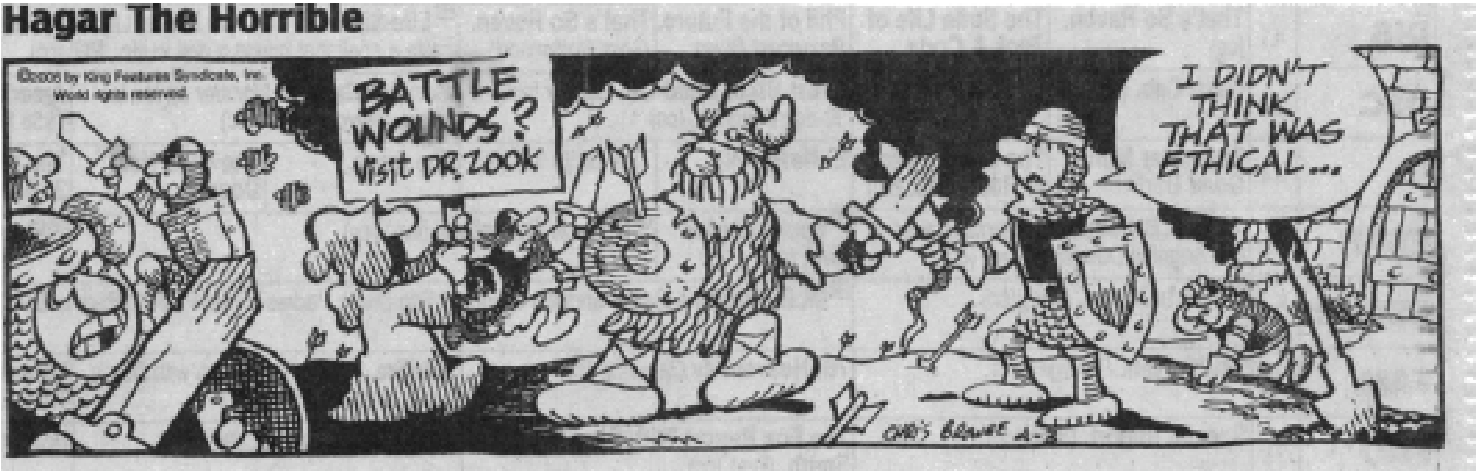
\includegraphics[width=5in]{./figures/DrZook.pdf} 
   \caption{Dr. Zook's advertising - at one time the medical profession thought that advertising was an unprofessional and tasteless business practice; that thought has changed.}
   \label{fig:drZook}
\end{figure}

Figure~\ref{fig:drZook} is a humorous perspective on medicine and its relationship to society.  The medical profession's mission is the amelioration of injury and illness; they expect to be paid, but even though physicians directly advertise I suspect that the soldier's shock is about the "in-your face" nature of Dr. Zook's approach.  Dr. Zook appears to be opportunistic, and I suspect the cartoonist intended that allegorical tone. The point of the figure in this seminar is that ethics is a concern in our daily lives.

\begin{figure}[h!] %  figure placement: here, top, bottom, or page
   \centering
   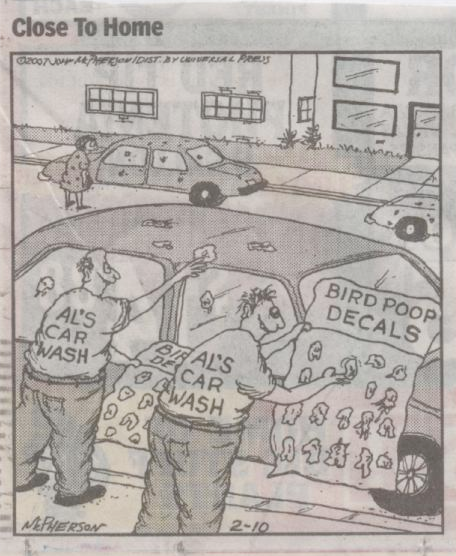
\includegraphics[width=5in]{./figures/Poop_on_car_ethics.pdf} 
   \caption{Guerilla advertising; engineering equivalent is planned obsolesce in order to obtain future work.}
   \label{fig:poop_on_car_ethics}
\end{figure}

Figure~\ref{fig:poop_on_car_ethics} is a similar example of ``in-your-face'' promotion of a business.  The engineering equivalent would be to damage public structures to obtain engineering services, or to intentionally design shortened life spans of engineered things, planned obsolesce is common in product engineering, but should never be part of a system engineered for the public.  Planned obsolesce is not the same as things wearing out and needing maintenance and replacement -- but if a choice is made for the purpose of additional business it is probably unethical.
\subsection*{A Fable}
These issues are quite timeless.  Consider fables.  Fables are very simple allegorical stories originally invented as a form of political criticism and as a tool to teach cultural values.
One such fable is that of Mercury and the Woodcutter.

\begin{em}
"A Woodsman was felling a tree on the bank of a river, when his axe, glancing off the
trunk, flew out of his hands and fell into the water. As he stood by the water's edge
lamenting his loss, Mercury appeared and asked him the reason for his grief. On learning
what had happened, out of pity for his distress, Mercury dived into the river and, bringing
up a golden axe, asked him if that was the one he had lost. The Woodman replied that it
was not, and Mercury then dived a second time, and, bringing up a silver axe, asked if
that was his. "No, that is not mine either," said the Woodman. Once more Mercury dived
into the river, and brought up the missing axe. The Woodman was overjoyed at
recovering his property, and thanked his benefactor warmly; and the latter was so pleased
with his honesty that he made him a present of the other two axes. When the Woodman
told the story to his companions, one of these was filled with envy of his good fortune
and determined to try his luck for himself. So he went and began to fell a tree at the edge
of the river, and presently contrived to let his axe drop into the water. Mercury appeared
as before, and, on learning that his axe had fallen in, he dived and brought up a golden
axe, as he had done on the previous occasion. Without waiting to be asked whether it was
his or not, the fellow cried, "That's mine, that's mine," and stretched out his hand eagerly
for the prize: but Mercury was so disgusted at his dishonesty that he not only declined to
give him the golden axe, but also refused to recover for him the one he had let fall into
the stream."
\end{em}

Let us ask ourselves some simple questions about the fable.
\begin{enumerate}
\item What is the �moral� or lesson of this fable?
\item Does this fable have any relationship to ethical situations (of course, but what?)
\item What were the consequences of the second woodsman�s �unethical� behavior?
\end{enumerate}

To summarize to this point.  Ethics is crucial to how engineers do their jobs; there is a compelling economic argument for ethical behavior in the context of corruption; and the issue is timeless - it plagued ancient people as well as ourselves; and finally, ethical theories suggest that there will, at times, be conflicts or dilemmas and some reasoning tool is needed to select a subsequent action.   The fable itself is the ancient equivalent of today's codes of ethics -- it was intended to guide people into making ethical (and civilized) choices.

Why a code of ethics?   By analogy consider that soldiers, police, firefighters, EMTs etc. are expected to perform in very high-stress situations with practically no time to think.  In their work, they endure nearly continuous training to function in a manner to ensure high-probability of correct response.   If patterns of failure are detected, the training is changed.  Code of ethics serves a similar purpose.
The codes provide guides to behave to an ethical issue (dilemma) in a manner to ensure a high-probability of correct response.  

Figure~\ref{fig:IP_ethics} is a humorous look at balancing the public good with the need to document ethical preparation.  In the comic, the ethical compliance software (a copyrighted piece of intellectual property) is shared without thought among colleagues at different firms.  The act of copying benefits the public (presumably by increasing collective ethical behavior) but it is unethical in that the original developer of the software is economically damaged.  While intended as humor, the same situations arise frequently in engineering -- fortunately our codes-of-ethics are free (for the price of a download).

\begin{figure}[h!] %  figure placement: here, top, bottom, or page
   \centering
   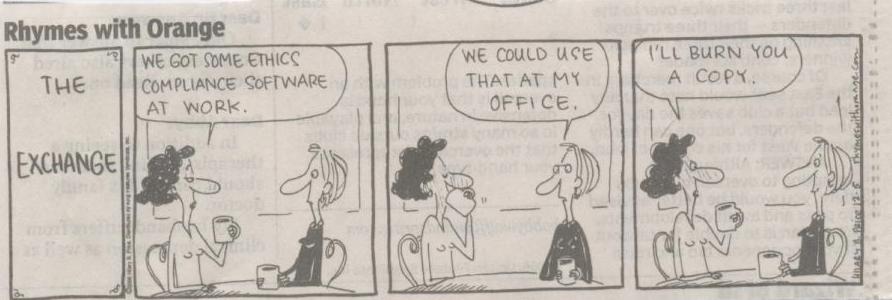
\includegraphics[width=5in]{./figures/IP_ethics.pdf} 
   \caption{Intellectual property ethics -- the situation depicted may be illegal if the software is not governed by GPL type license.}
   \label{fig:IP_ethics}
\end{figure}

The National Society of Professional Engineers (NSPE) is one example of a code of ethics.  The discipline specific codes of ethics are essentially clones of the NSPE code.  The ethics section of the Texas Engineering Practices Act is also a nearly verbatim copy of the NSPE act - except that since the Act is legislation, it does have the force of "law" behind it - in essence an unethical practice of engineering in Texas is also illegal.